\section{Model checkers}

The choice of an appropriate model checker is a crucial part of this work,
as it is the backend responsible for verifying the absence of deadlocks.
Fortunately, several model checkers have been developed for analyzing Petri nets.

The \acrfull{MCC} \cite{khhjp2021} organized at the Sorbonne University in Paris
is a great source for state-of-the-art model checkers.
It is an annual competition where submitted model checkers are run on a series of
Petri net models from academia and industry\footnote{\url{https://mcc.lip6.fr/2023/models.php}}.
These models have been contributed by many individuals over a period of more than a decade
and the total number of benchmarks has grown steadily as new models have been added.

Every year, the benchmarks include \acrfull{P/T nets}, i.e. Petri nets, and \acrfull{CPN}.
The number of places in the nets can range from a dozen to more than 70000 and transitions
can range from less than a hundred to more than a million.
This highlights the broad applicability of the model checkers that take part in the competition.

The results are published on the official website (see for instance \cite{mcc:2022}) and consist of:

\begin{enumerate}
  \item a list of the qualified tools that participated,
  \item the techniques implemented in each of the tools,
  \item a section dedicated to detailing the experimental conditions under which the contest took place
        (the hardware used and the time necessary to complete the runs),
  \item the results in the form of tables, plots, and even the execution logs of each program,
  \item a list of winners for each category,
  \item an analysis of the reliability of the tools based on the comparison of the results.
\end{enumerate}

A brief look at the slides of the 2022 edition\footnote{\url{https://mcc.lip6.fr/2022/pdf/MCC-PN2022.pdf}}
reproduced in Fig. \ref{fig:mcc2022-tools} illustrates
that several model checkers have demonstrated uninterrupted participation,
with notable examples including:

\begin{itemize}
  \item \acrfull{TAPAAL} maintained by the Aalborg University
        in Denmark\footnote{\url{https://www.tapaal.net/}},
        winner of a gold medal in the 2023 edition.
  \item \acrfull{LoLA} maintained by the University of Rostock
        in Germany\footnote{\url{https://theo.informatik.uni-rostock.de/theo-forschung/tools/lola/}},
        winner in previous editions and a base for other models.
  \item ITS-tools \cite{thierrymieg:hal-02104373},
        which was also combined with \acrshort{LoLA} and won medals
        in 2020\footnote{\url{https://github.com/yanntm/its-lola}}.
\end{itemize}

\begin{figure}[!htb]
  \centering
  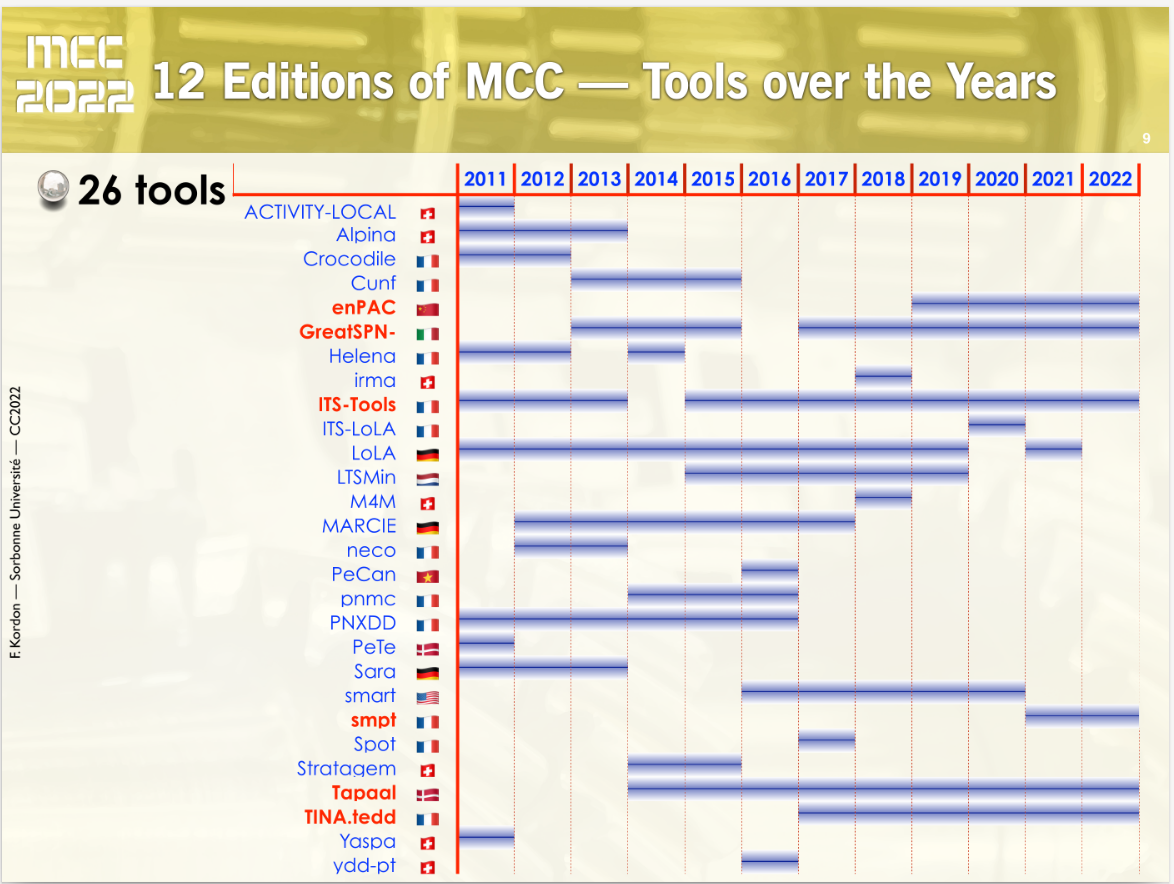
\includegraphics[width=\linewidth]{mcc2022-tools.png}
  \caption{Model checker participation in the MCC over the years.}
  \label{fig:mcc2022-tools}
\end{figure}

These observations collectively indicate
the maturity and vibrancy of the model checker community.
The establishment of a well-developed tool landscape,
fostered by international collaboration and the open-source dissemination of results, benchmarks, and techniques,
presents a valuable opportunity for leveraging these tools within the realm of software development.
Specifically, in the context of integrating them as backends for a language-specific translator
that takes care of automating the Petri net model creation process.
By capitalizing on the academic efforts invested in the model checkers,
increased safety and reliability in software projects can be achieved.
